\documentclass{article}
\usepackage[T1]{fontenc}

\usepackage{pgfplots}
\usepgfplotslibrary{groupplots}
\pgfplotsset{compat=1.5}

\begin{document}
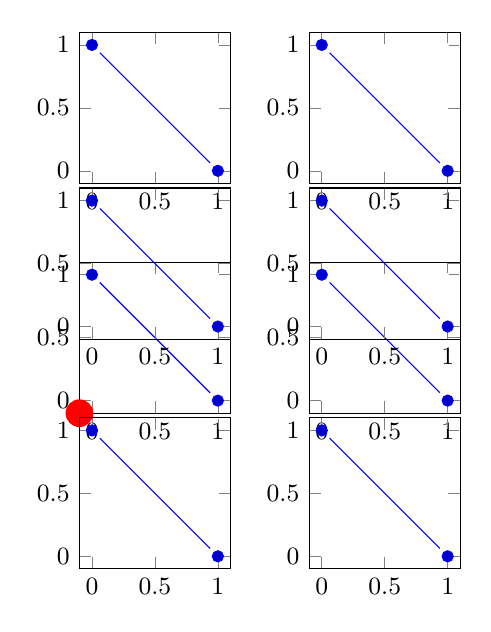
\begin{tikzpicture}[shorten >=4pt,shorten <=4pt]
  \begin{groupplot}[
  	group style={group size=2 by 2,
		group name=XYZ,
	},
    height=3.5cm,width=3.5cm,/tikz/font=\small]
    \nextgroupplot% 1
    \addplot coordinates {(0,1) (1,0)};
    \nextgroupplot% 2
    \addplot coordinates {(0,1) (1,0)};
    \nextgroupplot% 3
    \addplot coordinates {(0,1) (1,0)};
    \nextgroupplot% 4
    \addplot coordinates {(0,1) (1,0)};
  \end{groupplot}

\FIXIT
\fill[red] (XYZ c1r2.south west) circle (5pt);

  \begin{groupplot}[
  	% this here fails: 
  	at={(XYZ c1r2.south west)},
	anchor=above north west,
	% it works if I move it into the first group plot, though
  	group style={group size=2 by 2},
    height=3.5cm,width=3.5cm,/tikz/font=\small]
    \nextgroupplot[
	]% 1
    \addplot coordinates {(0,1) (1,0)};
    \nextgroupplot% 2
    \addplot coordinates {(0,1) (1,0)};
    \nextgroupplot% 3
    \addplot coordinates {(0,1) (1,0)};
    \nextgroupplot% 4
    \addplot coordinates {(0,1) (1,0)};
  \end{groupplot}
\end{tikzpicture}

\end{document}
